  \documentclass{standalone}
  \usepackage{amsmath}
  \usepackage{amsfonts}
  \usepackage{tikz}
  \usepackage{tikz-3dplot}
  \usepackage{pgfplots}
  \usepackage{pst-plot}
  \pgfplotsset{compat=1.18} % version number
  \usepackage{physics}
  \usepackage[outline]{contour} % glow around text
  \begin{document}
  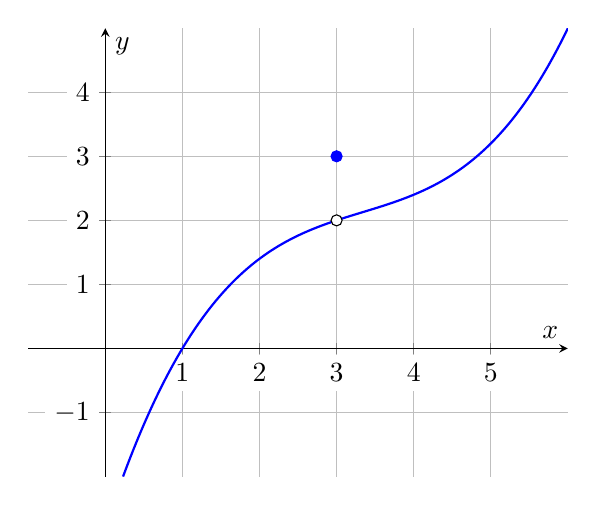
\begin{tikzpicture}

    \pgfplotsset{soldot/.style={color=blue,only marks,mark=*},
             holdot/.style={color=black,fill=white,only marks,mark=*},
             compat=1.12}
    \begin{axis}[   grid=both,
                    axis lines=middle,
                    ticklabel style={fill=white},
                    xmin=-1,xmax=6,
                    ymin=-2,ymax=5,
                    xtick={1, 2, 3, 4, 5},
                    ytick={-1, 1, 2, 3, 4},
                    xlabel=\(x\),ylabel=\(y\),
                    samples=200
                ]
        \addplot[domain=0.23:6, blue, thick] {0.1*(x*x*x - 10*x*x + 37*x - 28)};
        \addplot[holdot] coordinates{(3, 2)};
        \addplot[soldot] coordinates{(3, 3)};
    \end{axis}
  \end{tikzpicture}
  \end{document}
